%NMF (1.6 TB)
%MPI 50 nodes 66s
%100 nodes 45s
%300 nodes 30s
%spark (1.6 TB)
%50 nodes 710s
%100 nodes 457s
%300 nodes 215s
%PCA (2.2 TB)
%MPI 100 nodes 94s
%300 nodes 60s
%500 nodes 56s

%spark (2.2 TB)
%100 nodes 15:58
%300 nodes 14:30
%500 nodes 20:30

%PCA spark (7.9 TB)
%1522 nodes 01:12:46
%PCA MPI 160s


\begin{figure*}[th!]
\begin{center}
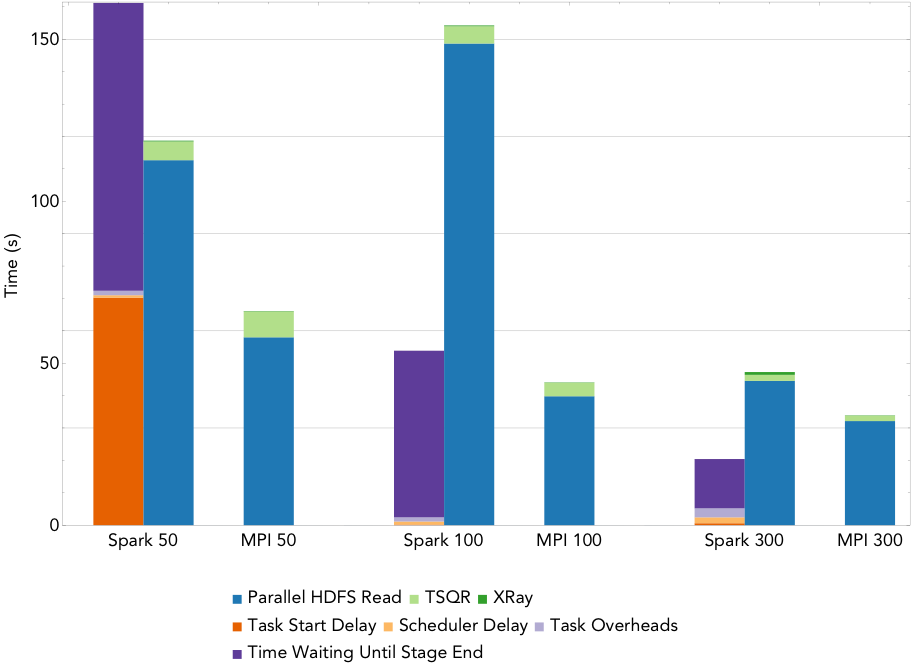
\includegraphics[width=\textwidth]{fig/nmf_run_times.png}
\caption{Running time breakdown of NMF on the 1.6TB Daya Bay matrix at 
node counts of 50, 100, and 300.}
\label{fig:nmfrt}
\end{center}
\end{figure*}

\begin{figure}[h]
\centering
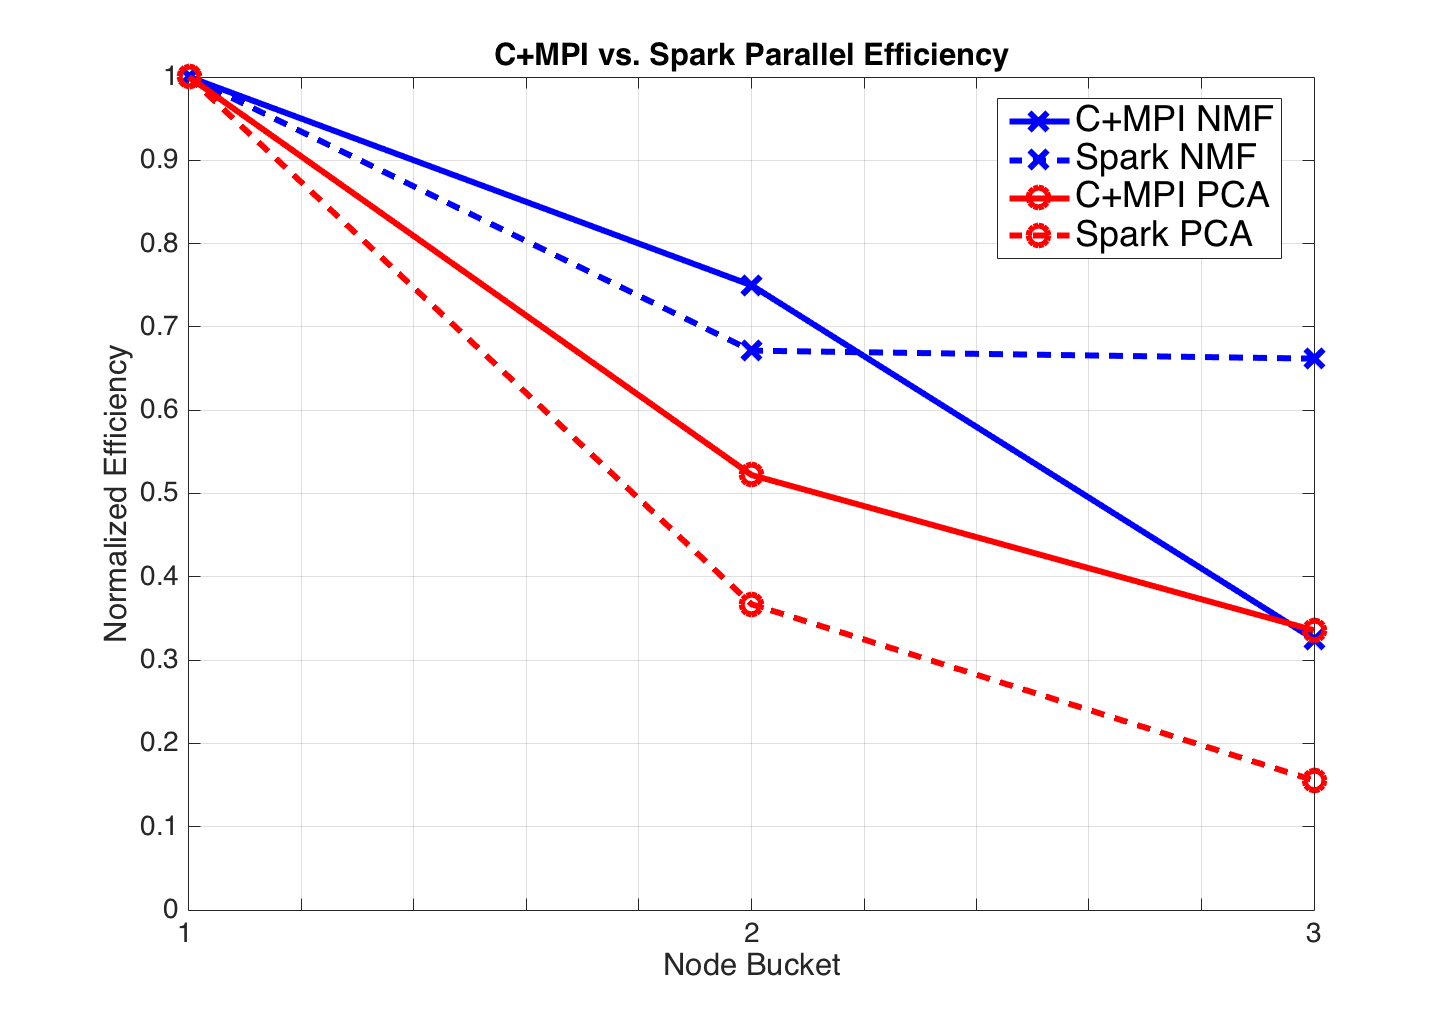
\includegraphics[width=\textwidth]{fig/peff.png}
\caption{Comparison of parallel efficiency for C+MPI and Spark. The x-axis label ``Node Bucket'' refers to the node counts. For NMF these are 50, 100, and 300 nodes (left to right) and 100, 300, and 500 nodes for PCA.}
\label{fig:peff}
\end{figure}

\begin{table}[t]
\centering

\begin{tabular}{|c|c|c|c|c|c|} \hline
Algo & Size & \# Nodes & MPI Time (s) & Spark Time (s)\\ \hline
\multirow{3}{*}{NMF} & \multirow{3}{*}{1.6 TB} & $50$ & $66$ & $278$\\
{} & {} & $100$  & $45$ & $207$\\
{} & {} & $300$ & $30$ & $70$\\ \hline
\multirow{4}{*}{PCA} & \multirow{3}{*}{2.2 TB} & 100 & 94 & 934\\
 {} & {} & 300 & 60 & 827\\
 {} & {} & 500 & 56 & 1160\\ \cline{2-5}
 {} & {16 TB} & {MPI: 1600 Spark: 1522} & 160 & 4175 \\ \hline
\end{tabular}
\caption{{Summary of Spark and MPI running times.}}
\label{tab:matrix}
\end{table}

\subsection{NMF on Daya Bay}
The separable NMF algorithm we implemented fits nicely into a data parallel programming model. After the initial parallel TSQR the remainder of the algorithm can be computed sequentially. The Daya Bay dataset is especially amenable to this approach due to the extreme aspect ratio of the dataset and a desired rank of $10$.
\subsubsection{C+MPI vs. Spark}
The TSQR algorithm used performs a single round of communication using a flat binary tree and given that the number of columns is very small the NMF algorithm is entirely I/O bound. Figure \ref{fig:mpinmf} shows the running time breakdown of the MPI version of NMF at 50 nodes, 100 nodes, and 300 nodes. The running time for NMF is overwhelmingly dominated by reading the input and, to a lesser degree, the the row-major to column-major transpose. In comparison, TSQR and~\textsc{XRay} have negligible running times. Figure \ref{fig:mpinmf} shows that the HDF5 read time (in green) does not scale linearly with the number of nodes and is the primary source of inefficiency -- this is due to saturating the system bandwidth for 72 OSTs. The transpose operation (in red) scales linearly with the number of nodes but represents overhead that can be avoided entirely. ~\textsc{XRay} is the sequential bottleneck and costs ~$100$ms at all node counts. TSQR only improves by tens of milliseconds taking $501$ms, $419$ms, and $378$ms at 50, 100, and 300 nodes, respectively. The poor TSQR scaling can be attributed to hitting a communication bottleneck. The TSQR  binary tree is expensive for small matrices especially using flat-MPI. We did not tune our TSQR reduction tree shapes or consider other algorithms since TSQR is not the limiting factor to scalabilty. These results illustrate the importance of I/O scalability when performing terabyte-scale data parallel analytics on a high-performance architecture using MPI.

Figure \ref{fig:nmfspark} illustrates the running time breakdown for Spark NMF on 50, 100, and 300 nodes. Unlike C and MPI, Spark incurs significant overhead for task scheduling, task start delays and idle time due to Spark stragglers. For the 50 node run we configured Spark to use double the number of partitions as physical cores because we encountered out-of-memory errors for fewer partitions. The number of partitions was not doubled for the 100 and 300 node runs. Similar to the C and MPI results, most of the running time is dominated by I/O and Spark overheads with a small amount of time spent in TSQR and \textsc{XRay}. The Spark version does not include an explicit transpose, the Breeze library performs it if necessary when making a call to optimized BLAS during TSQR. Figure \ref{fig:nmfspark} shows that Spark NMF exhibits good strong scaling behavior up to 300 nodes.  Even though NMF is entirely data parallel and suitable for Spark, we observed a $4\times$, $4.6\times$, and $2.3\times$ performance gap on 50, 100, and 300 nodes, respectively, between Spark and MPI.

Figure \ref{fig:peff} shows the parallel efficiency results which are normalized to the 50 node running time of the respective parallel frameworks. MPI NMF is completely dominated by I/O and the results are primarily indicative of scaling issues in the I/O subsystem. Spark NMF displays good scaling with more nodes and this is reflected in the parallel efficiency. However, the scaling is due to decreases in Spark overhead.

\subsubsection{Science Interpretation}
We are currently investigating the results of the NMF decomposition. Preliminary analysis of the results indicates that we will need to augment the input data with non-linear feature descriptors (Kernel methods) to make the input signals invariant to rotations and translations. Our eventual goal is to learn event-specific classifiers from the coefficients of the basis vectors. The classification will enable us to accomplish the final goal of segmenting and labeling the timeseries. While successfully implementing the entire pipeline is somewhat out of scope for this submission, the fact that we have determined basis vectors from the TB-sized dataset will enable us to explore more advanced methods in the near future.

\begin{figure*}[th!]
\centering
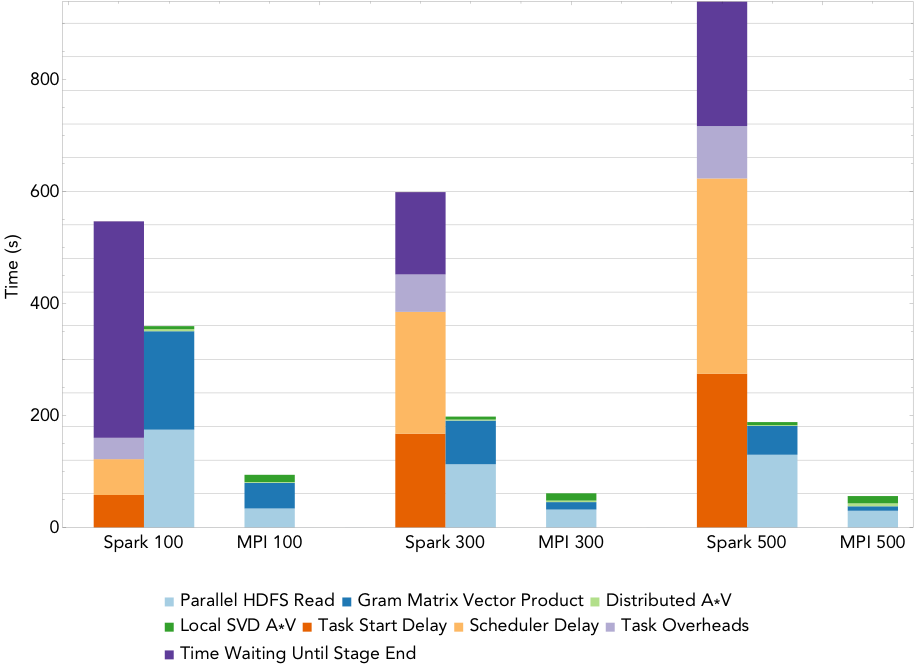
\includegraphics[width=\textwidth]{fig/ocean_pca_times.png}
\caption{Running time breakdown of PCA on the 2.2TB Ocean matrix at node counts of 100, 300 and 500.}
\label{fig:pcart}
\end{figure*}

\begin{figure}[th!]
\centering
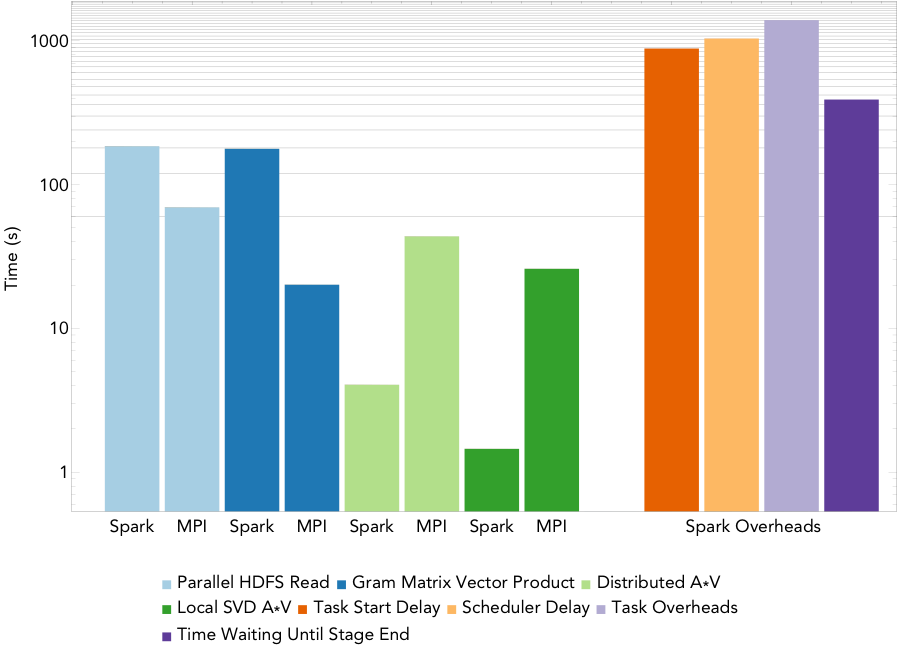
\includegraphics[width=\textwidth]{fig/hero_pca_times.png}
\caption{Running time comparison of the Spark and MPI implementations of PCA on the 16TB Atmosphere matrix.}
\label{fig:hero}
\end{figure}

\subsection{PCA on Climate}

PCA is an iterative algorithm which requires an SVD of the data matrix in order to find its top-$20$ left singular vectors. The main kernel of this algorithm is a distributed matrix-vector product at every iteration. Since matrix-vector products are data parallel, the PCA algorithm also fits into the Spark model. The additional requirement for PCA is that the data matrix needs to be cached in memory on Spark to avoid I/O at each iteration.

\subsubsection{C+MPI vs. Spark}
%The C and MPI version reads the dataset from a single HDF5 file, computes a rank-$k$ eigenvalue decomposition, EVD, ($V\Lambda V^T$) of the Gramian matrix $A^TA$ in parallel, performs a parallel matrix-matrix multiplication ($AV$) and, finally, a sequential singular value decomposition of $AV$. Once again, the matrix is partitioned into a 1D-block row decomposition. We use arpack-ng \cite{Lehoucq97} to compute the EVD which requires a user-defined function to perform matrix-vector products. We do this by first broadcasting the Lanczos vector $x$ to all processors and compute a local matrix-vector product. This results in a vector $y = Ax$ distributed across different processors, from which the vector $z = A^Ty$ can be computed. $z$ is formed by computing partial matrix-vector products using locally stored blocks of $A$ and $y$, which are then globally summed using an \verb+MPI_Allreduce+. This process is repeated until the Lanczos method converges -- we set the tolerance to $10^{-13}$. After convergence the $k$ eigenvectors just computed are broadcasted to all processors which compute partial matrix-matrix products that are globally summed. Finally,  we compute a sequential SVD to obtain the top-$k$ left singular vectors of $A$. 
Figure \ref{fig:mpipca} shows the running time breakdown results for PCA on 100, 300, and 500 nodes. I/O is a significant bottleneck and does not exhibit the scaling observed for NMF in Figure \ref{fig:mpinmf}. However, the absolute I/O time for NMF and PCA are consistent which suggests that the I/O bandwidth is saturated for the stripe size used for the Daya Bay and Ocean datasets. The Gram matrix-vector products are a significant portion of the running time but scale linearly with the number of nodes. The matrix-matrix product ($AV$) does not scale due to a communication bottleneck. The bottleneck is because we compute a rank-$20$ PCA which makes communicating $V$ very expensive. This cost grows with the number processors since it is entirely latency dominated. The final SVD of $AV$ is a sequential bottleneck and does not scale. Unlike NMF the sequential bottleneck in PCA is significant and future implementations should perform this step in parallel.

Figure \ref{fig:sparkpca} shows the scaling and running time breakdown of the Spark PCA implementation for 100, 300, and 500 nodes. The Gram matrix-vector products scale linearly with the number of nodes however this is outweighed by inefficiencies in Spark. At this scale, Spark is entirely bottlenecked by scheduler delays, task overhead and Spark straggler delay times. Task overhead consists of deserializing a task, serializing a result and writing and reading shuffle data. The Spark scheduling delay and task overhead time scales inversely with the number of nodes. This is likely due to the centralized scheduler used in Spark. PCA is a data parallel algorithm, however, its iterative nature stresses the Spark scheduler since many tasks are launched during each iteration. Under this workload we observed a 10.2$\times$, 14.5$\times$, and 22$\times$ performance gap on 100, 300, and 500 nodes, respectively, between Spark and MPI. The running time disparity between $AV$ products and sequential SVD can be attributed to the use of single-threaded BLAS for MPI and multi-threaded BLAS for Spark.

Figure \ref{fig:peff} shows the parallel efficiency of MPI PCA and Spark PCA. In the PCA case we observed that the MPI version hits an I/O bottleneck, a communication bottleneck in the $AV$ product and a sequential bottleneck in SVD($AV$). All of these are limiting factors and introduce inefficiencies to MPI PCA. Spark PCA is less efficient that MPI PCA due to scheduler delays, task overhead and straggler effects. The scheduler delays are more prominent in PCA than in NMF due to the larger number of tasks. NMF makes a single pass over the data whereas PCA makes many passes over the data and launches many tasks per iteration.
% \begin{figure}[t]
% 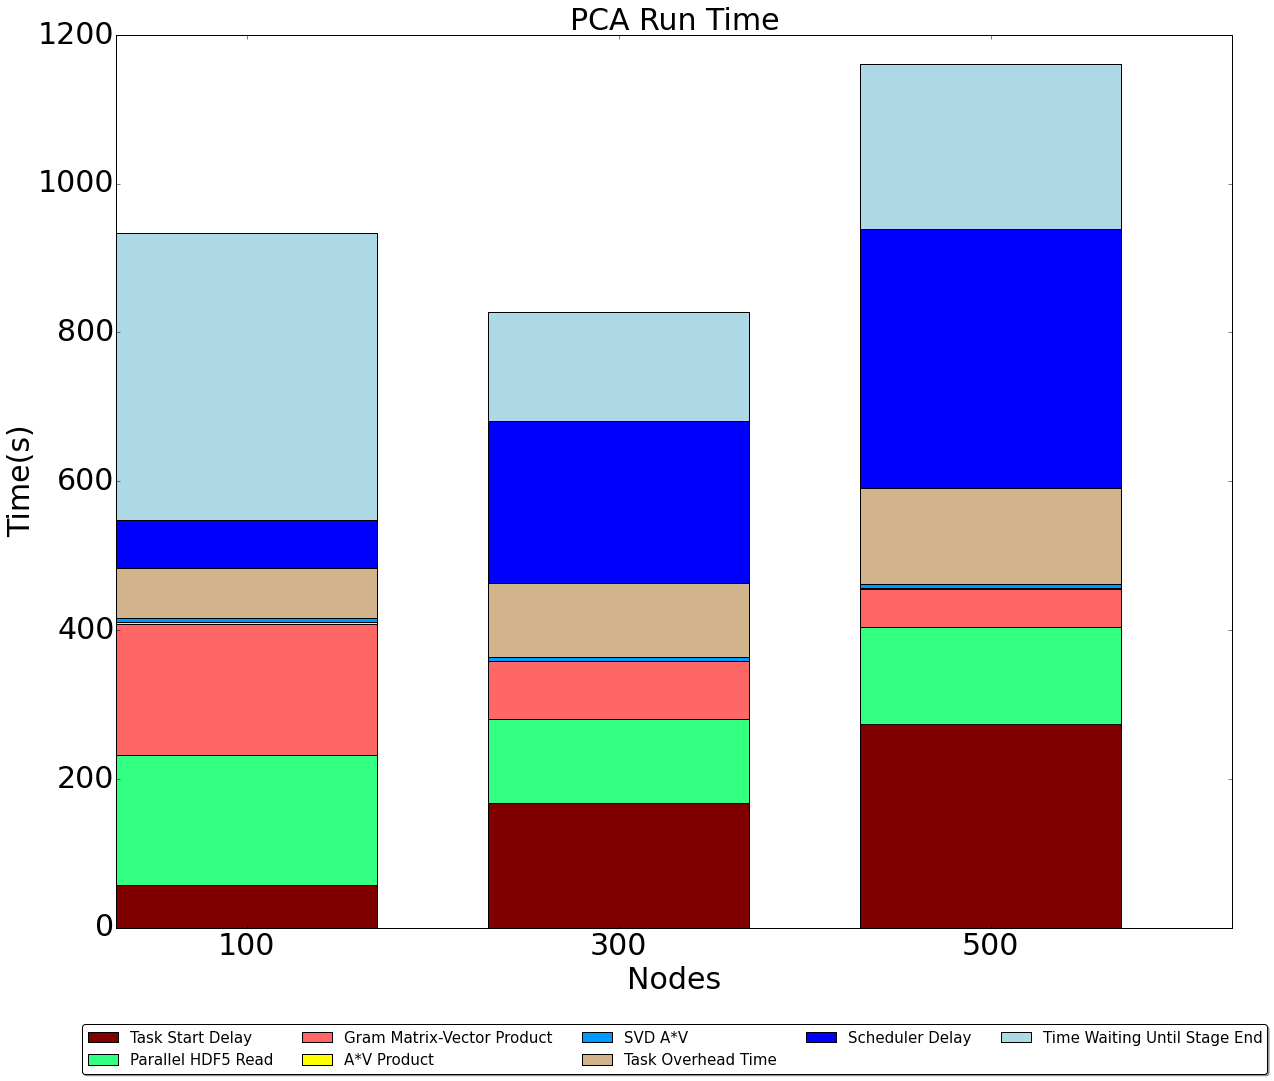
\includegraphics[width=.5\textwidth]{fig/spark_pca.png}
% \end{figure}


% \begin{figure}[t]
% 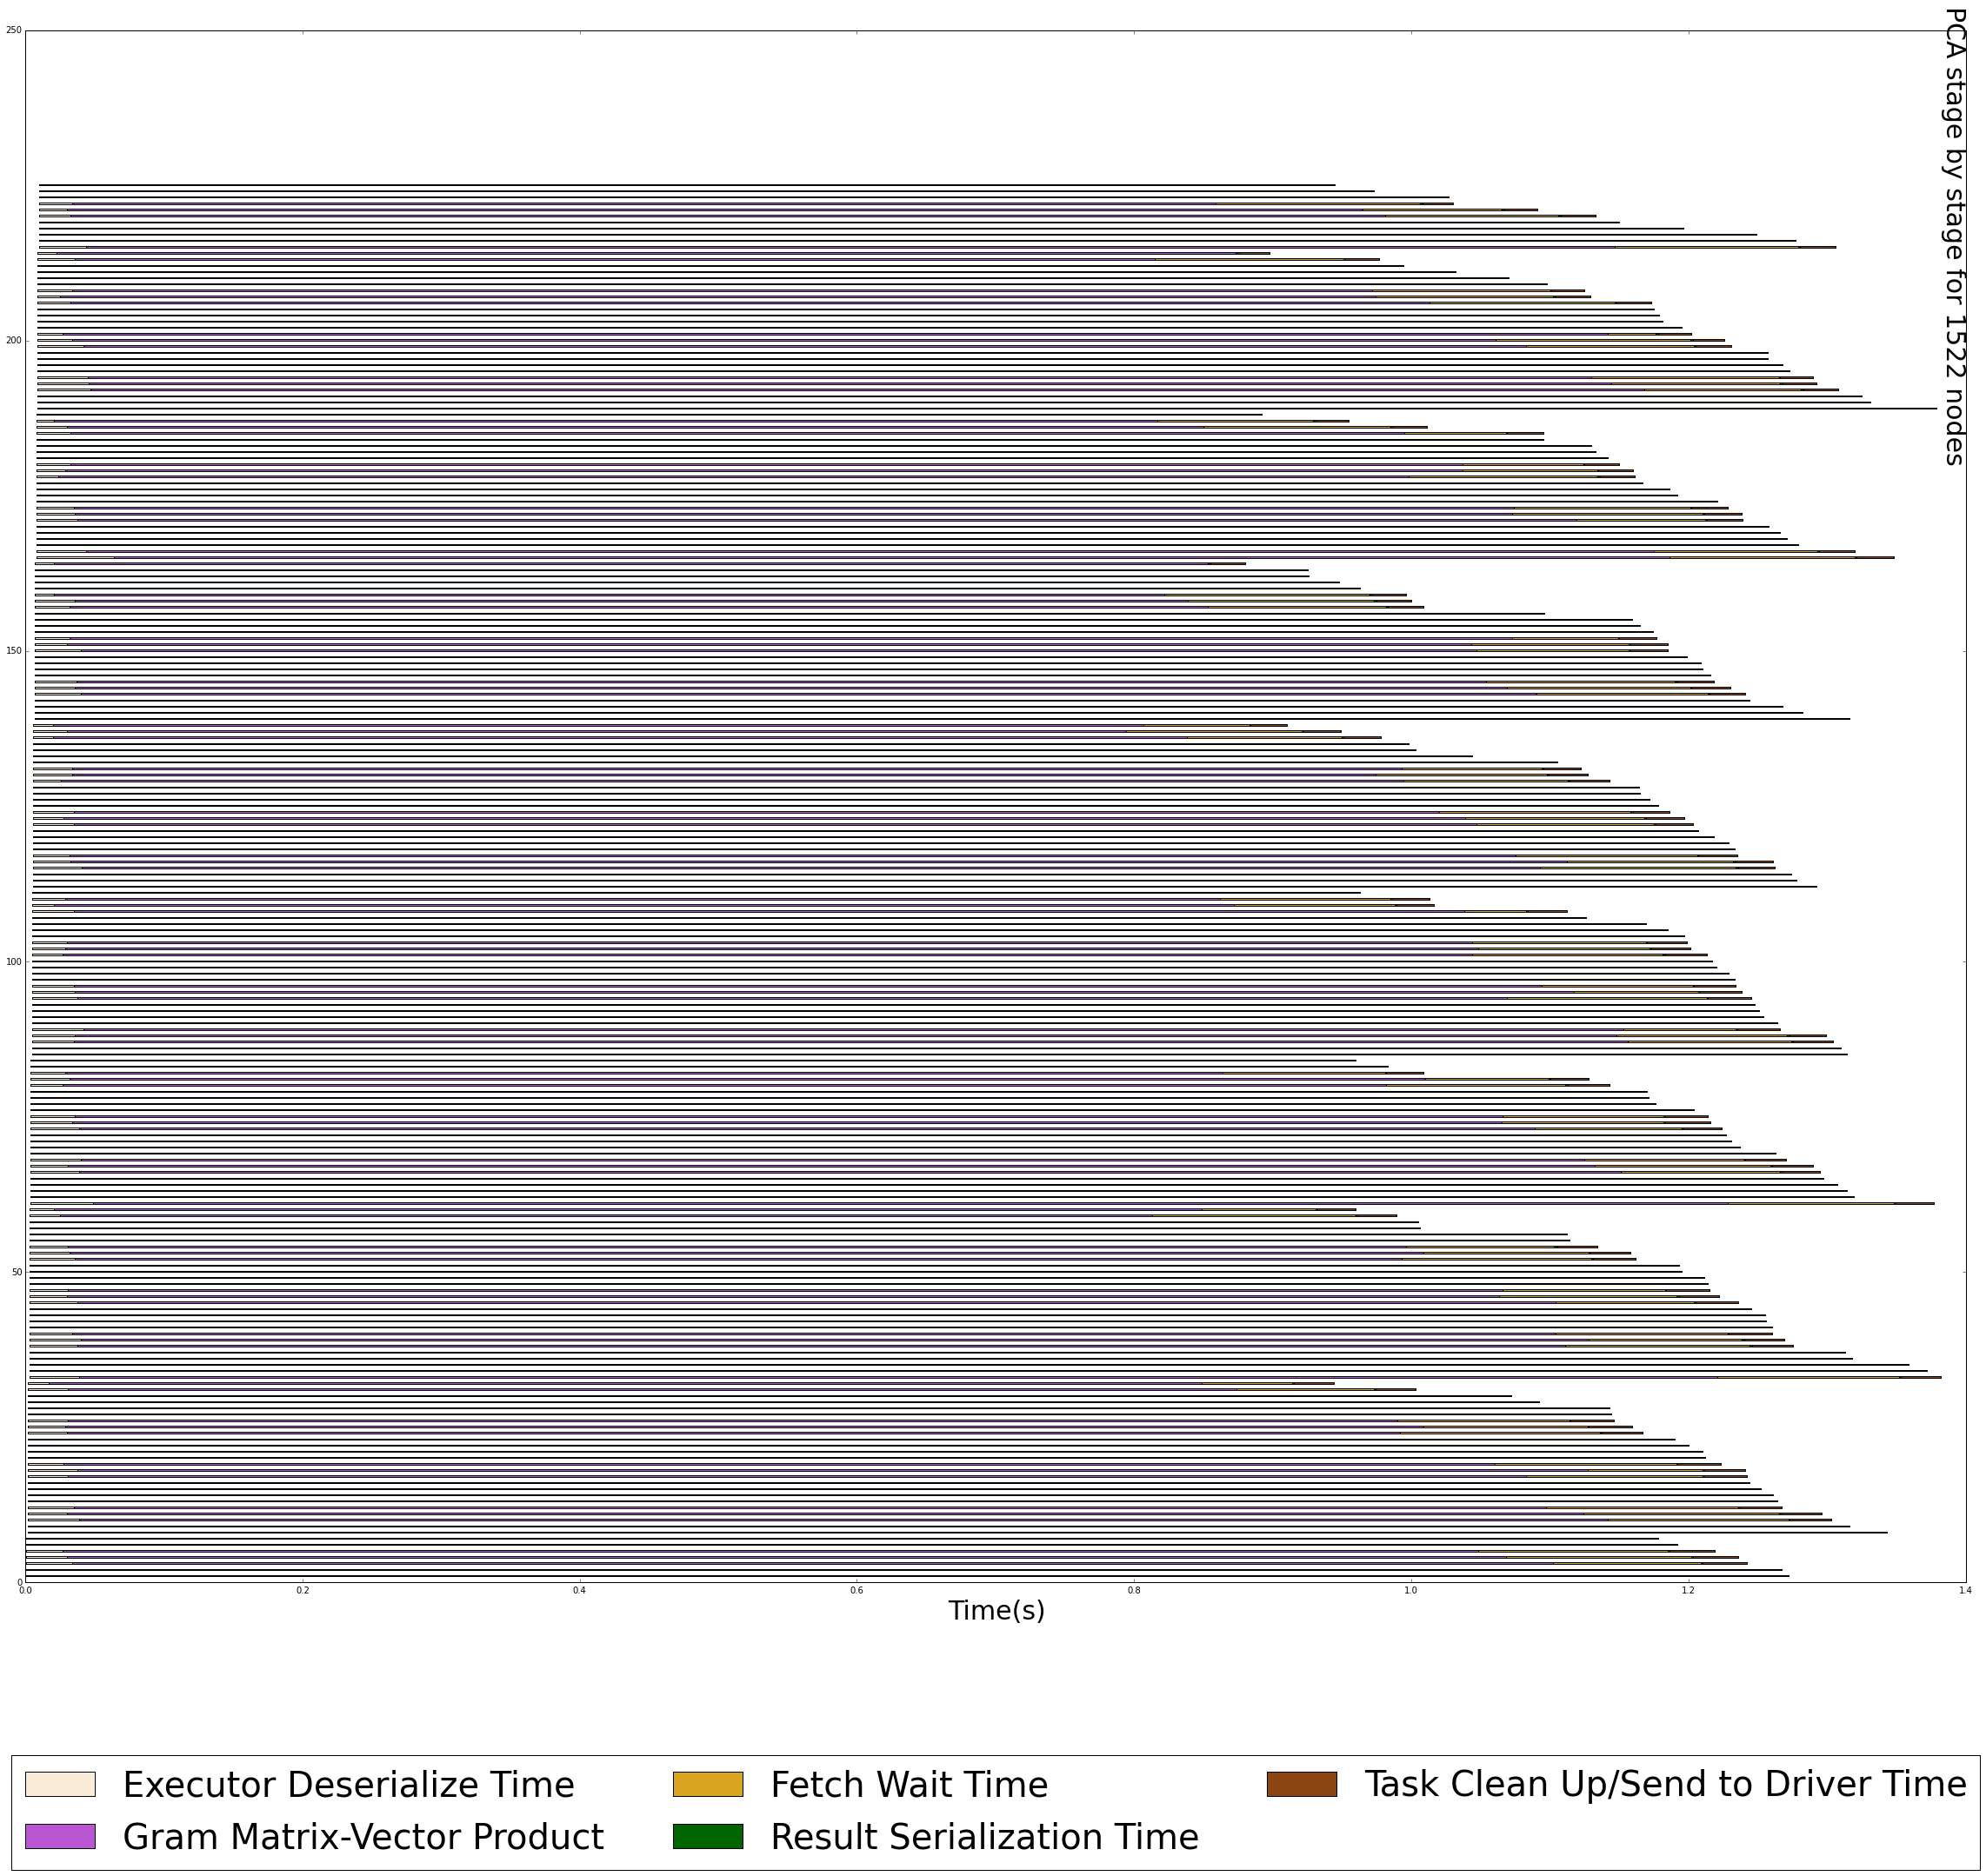
\includegraphics[width=.5\textwidth]{fig/stage_8_hero_run.png}
% \end{figure}

%\textcolor{blue}{parallel efficiency, stacked bar graph of running time.}
\subsubsection{PCA Hero Run}

We used all 1600 Cori nodes to perform PCA on the 16TB CAM5 atmospheric dataset. In order to complete this test in a reasonable amount of time, we fix  the number of iterations for the EVD of $A^TA$ to $70$ iterations. MPI PCA was able to complete this run in $160s$. Unfortunately we were unsuccessful at launch Spark on $1600$ nodes and after many attempts we reduced the number of nodes to $1522$. Once the node count was decreased Spark PCA successfully completed the run in $4175s$. Figure \ref{fig:hero} shows the head-to-head running time comparison of the full-system run. The Gram matrix-vector products are an order of magnitude more costly in Spark. We noticed that the tree-aggregates were very slow at full-system scale and are the likely cause of slow Gram matrix-vector products. The $AV$ and SVD in Spark are much faster than MPI due to use of multiple OpenBLAS threads. Finally, we observed that the Spark overheads were an order of magnitude more than the communication and computation time.

\subsubsection{Science Interpretation}
For the 2.2TB oceanic dataset, the first two temporal EOFs, {corresponding to right singular vectors}, fully capture the annual cycles. The remaining time series show abrupt changes due to the 1983 ENSO, and more significantly, the record-breaking ENSO of 1997--98. The intermediate modes contain a complex interplay of various timescales, which is currently under investigation. The spatial EOFs, corresponding to $U_k$, show the relative dominance of the Indian Ocean Dipole and the classic warm pool--cold tongue patterns of ENSO at various depths below the ocean surface. Because of the 3D nature of the EOFs, we are able to see that the dynamic near the thermocline is most dominant, rather than that closer to the surface. Further, there are several smaller scale features that have a strong influence at different depths. Work is on-going to understand the nature of these different spatial patterns and the factors that influence their relative dominance.

\subsection{CX on Mass-spec Imaging}
\begin{table}[t]
\centering
\begin{tabular}{|c|c|c|c|} \hline
Algo & Size & \# Nodes & Spark Time (s)\\ \hline
\multirow{3}{*}{CX} & \multirow{3}{*}{1.1 TB} & $60$ & $1200$\\
{} & {} & $100$  & $784$\\
{} & {} & $300$ & $542$\\ \hline
\end{tabular}
\caption{Spark CX running times}
\label{tab:cxscale}
\end{table}
Much like PCA, the CX decomposition requires a parallel Gramian multiply, a distributed matrix-matrix product and a randomized SVD in order to compute extremal columns of $A$. CX is applied to the 1.1TB MSI dataset stored as a file in native Spark Parquet format. Table \ref{tab:cxscale} shows the running times and scaling behavior of Spark CX. We found that Spark exhibited good scaling for the range of nodes tested and attained speedups of $1.5\times$ and $2.2\times$ on 100 and 300 nodes, respectively. The corresponding parallel efficiencies are 90\% for 100 nodes and 44\% for 300 nodes. These results show that the behavior of CX is similar to that of PCA, which is due to the overlap in their linear algebra kernels.
\subsubsection{Science Interpretation}
 The CX decomposition selected ions in three narrow regions of $m/z$. Among those ions identified as having significant leverage scores are ions at $m/z$ values of 439.0819, 423.0832, and 471.1276, which correspond to neutral losses of $\rm{CH_2}$, $\rm{CH_2O}$, and a neutral ``gain'' of $\rm{H_2O}$ from the 453.0983 ion.  These relationships indicate that this set of ions, all identified as having significant leverage scores, are chemically related.  That fact indicates that these ions may share a common biological origin, despite having distinct spatial distributions in the plant tissue.  

 \subsection{Summary of Spark vs. C+MPI performance comparison}
 \begin{table}[t]
\begin{center}
\begin{tabular}{|c|c|c|c|} \hline
Algo & \# Nodes & Gap with I/O & Gap without I/O\\ \hline
\multirow{3}{*}{NMF} & $50$ & $4\times$ & $21.2 \times$\\
{} & $100$  & $4.6\times$ & $14.9\times$\\
{} & $300$ & $2.3\times$ & $15.7\times$\\ \hline
\multirow{4}{*}{PCA} & 100 & $10.2\times$ & $12.6\times$\\
 {} & 300 & $14.5\times$ & $24.7\times$\\
 {} & 500 & $22\times$ & $39.3\times$\\ \cline{2-4}
 {} & {MPI: 1600 Spark: 1522} & $26\times$ & $43.8\times$\\ \hline
\end{tabular}
\end{center}
\caption{Summary of the performance gap between the MPI and Spark implementations.}
\label{tab:perfgaps}
\end{table}
We have demonstrated that matrix factorizations (which have traditionally been implemented using high-performance parallel libraries) can be implemented on Spark, and that Spark can run on large node counts on HPC platforms. By exploring the performance trade-offs of Spark matrix factorizations and comparing to traditional MPI implementations we have gained key insights into Spark's scalability. Table \ref{tab:perfgaps} summarizes the performance gaps between Spark and MPI which are $2\times - 25\times$ with I/O times and $10\times - 40\times$ without I/O times. Though the gaps may be large, our experiments indicated that Spark I/O scaling is comparable to MPI I/O scaling, that the computation scales well and that the primary bottlnecks are scheduler delays, straggler effects and task overhead times. If these bottlenecks can be alleviated, then Spark can close the performance gap and become a competitive, easy-to-use framework for data analytics on high-performance architectures.   

        
